\chapter{TKGE-PN模型实验与验证}
为了验证本文提出的TKGE-PN算法能够通过结合图路径和局部邻域信息实现对知识图谱中的长短距离依赖的综合学习,提高链路预测任务的性能表现,本文在两个基准数据集上对TKGE-PN进行了实验验证。TKGE-PN模型实验时采用的数据集、实验环境和评估策略和NATLP模型实验时完全一致,因此本章不再另行介绍。本章首先说明了用来对比的基线算法以及模型在两个数据集上的超参数设置,随后介绍了模型的整体实验结果并进行了深入的探究,最后通过消融实验对模型的关键设计进行了分析和讨论。

\section{实验方案设计}

\subsection{对比算法}

为了验证本文提出的TKGE-PN模型在链路预测任务上的有效性,在实验部分,本文将其与一些最具代表性的以及最先进的知识图谱嵌入模型进行了比较,主要包含以下几类:

(1)传统的知识图谱嵌入模型,时间和空间复杂度较低,包括基于翻译的模型TransE\upcite{TransE},RotatE\upcite{RotatE},基于张量分解的模型DistMult\upcite{DistMult},ComplEx\upcite{ComplEx},以及基于卷积神经网络的模型ConvE\upcite{ConvE}和ConvR\upcite{ConvR}。

(2)基于图神经网络的嵌入模型,主要学习图谱局部邻域结构进行知识图谱嵌入,包括R-GCN\upcite{R-GCN},CompGCN\upcite{CompGCN},KBGAT\upcite{KBGAT},HKGN\upcite{HKGN},SE-GNN\upcite{SE-GNN}以及MRGAT\upcite{MRGAT}。

(3)基于图路径的嵌入模型,利用知识图谱的图路径结构进行嵌入工作,包括RSN\upcite{RSN}和Interstellar\upcite{Interstellar}。 

(4)基于Transformer的嵌入模型,主要利用Transformer的表达能力进行链路预测,包括KG-BERT\upcite{KG-BERT},HittER\upcite{HittER},StAR\upcite{StAR}和Relphormer\upcite{Relphormer},以及本文先前提出的NALTP模型。

\subsection{模型超参数设置}

实验采用的超参数是通过网格搜索在验证集上进行评估后得出的。实验中,Path-Transformer图路径编码模块以及Neighbor-Transformer局部邻域编码模块分别由3层和4层Transformer编码层组成,多头注意力机制的头数为8,采用的实体和关系嵌入维度为320。在路径采样算法的设置上,两个数据集上路径采样的深度偏差权重$\alpha = 0.7$,度数偏差权重$\beta=0.1$,WN18RR数据集上采样路径的最大长度$T=4$,FB15k-237数据集上$T=3$。在掩蔽实体关系预测任务中,每个实体和关系有30\%的概率被特殊的掩蔽占位嵌入$e_{mask}$替换,20\%被其余随机实体和关系替换,50\%的概率维持不变。考虑到数据集中存在极小一部分节点度数极高的实体以及FB15k-237和WN18RR数据集在节点平均度数上的差异,实验对每个实体采样得到的图路径的最大数量进行了限制,在FB15k-237和WN18RR数据集上分别为50和12,这样的设置能够保证采样的图路径可以完全覆盖数据集中80\%以上实体的一阶邻域。

实验中采用了Adamax\upcite{Adamax}优化器结合动态学习率调整策略进行模型的训练。在总迭代次数的前10\%内,模型的学习率将从0线性提升到最高,并在剩余迭代次数内线性下降到0。在训练过程中,除了嵌入层以外的神经网络层的随机失活概率为0.65,嵌入层的随机失活概率为0.2。模型训练时在FB15K-237数据集上的总迭代次数为300,训练批次的大小为512,最大学习率为0.0011;而对于WN18RR数据集,总迭代次数为500,批处理大小为512,最大学习率为0.002。为了防止模型出现过度自信的现象,训练过程中以0.1的比率进行了标签平滑。模型使用的具体超参数参见表\ref{TKGE-PN_hyperparameter}。

\begin{table}[htbp]
    \renewcommand\arraystretch{1.5}
    \caption{TKGE-PN模型超参数设置}
    \centering
    \begin{tabular}{*{3}{c}}
      \toprule
      超参数 & FB15k-237 & WN18RR\\
      \midrule
      实体和关系嵌入大小  & 320 & 320 \\
      Path-Transformer网络层数& 3 & 3\\
      Neighbor-Transformer网络层数& 4 & 4\\
      嵌入层Dropout概率 & 0.2 & 0.2\\
      Transformer中的Dropout概率 & 0.65 & 0.65\\
      采样路径的最大长度&3 &4\\
      深度偏差权重& 0.7 & 0.7\\
      度数偏差权重& 0.1 & 0.1\\
      路径采样最大数量 &50&12\\
      训练批次大小 & 512 & 512\\
      总迭代次数& 300 & 500 \\
      最大学习率 & 0.001 & 0.02\\
      标签平滑比例 & 0.1 & 0.1\\
      \bottomrule
    \end{tabular}
    \label{TKGE-PN_hyperparameter}
  \end{table}

\section{实验结果与分析}

\subsection{整体实验结果分析}

不同模型在WN18RR数据集和FB15k-237数据集上的链路预测实验结果如表所示。和NATLP类似,TransE、RotatE、DistMult、ComplEx和ConvE在两个数据集上的实验结果直接选取文献\cite{49}中经过大量调参的最优结果。由于存在评估策略不当以及测试集数据泄露的问题,KBGAT的实验结果选取文献\cite{50}中经过修正后的结果。

\begin{table}[htbp]
    \begin{center}
        \caption{TKGE-PN实验结果}
        \renewcommand\arraystretch{1.5}
        \setlength{\tabcolsep}{5pt}
        \begin{tabular}{*{11}{c}}
            \toprule
            \multirow[vpos]{2}{*}[-0.8ex]{模型} & \multicolumn{5}{c}{WN18RR} & \multicolumn{5}{c}{FB15k-237}\\
            \cmidrule(lr){2-6}\cmidrule(lr){7-11}
            &MRR & MR & Hits@1 &Hits@3 & Hits@10&MRR & MR & Hits@1 &Hits@3 & Hits@10\\
            \midrule
            TransE&0.228&-&0.053&0.368&0.520&0.313&-&0.221&0.347&0.497\\
            RotatE&0.478&-&0.439&0.494&0.553&0.333&	-&0.240&0.368&0.522\\
            DistMult&0.452&-&0.413&0.466	&0.530	&0.343	&-	&0.250	&0.378	&0.531\\
            ComplEx&0.475&-&0.438	&0.490	&0.547	&0.348	&-	&0.253	&0.384	&0.536\\
            ConvE&0.442&-&0.411&0.451	&0.504&	0.339	&-&	0.248&	0.369	&0.521\\
            ConvR&0.475&-&0.443&	0.489&	0.537&	0.350&	-&	0.261&	0.385&	0.528\\
            \cmidrule{1-11}
            R-GCN & -&-&-&-&-&0.248&-&0.153&0.258&0.414\\
            CompGCN&0.479&3533&0.443	&0.494	&   0.546&	0.355	&197	&0.264	&0.390&	0.535\\
            KBGAT&0.412&1921&-&	-&	0.554	&0.157	&270	&-&	-&	0.331\\
            SE-GNN&0.484&3211&0.446&	0.509&	0.572	&0.365& 157	&0.271	&0.399	&0.549\\
            MRGAT&0.481&-&0.443&0.501&0.568&0.358	&-&0.266&0.386&0.542\\
            HKGN&0.487&2468&0.448&0.505&0.561&0.365&194&0.271&0.397&0.544\\
            \cmidrule{1-11}
            RSN&0.400&-&0.380	&-	&0.448&	0.280	&-	&0.202	&-	&0.453\\
            Interstellar&0.480&-&0.438	&-	&0.546	&0.320	&-	&0.233	&-	&0.508\\
            \cmidrule{1-11}
            KG-BERT&0.216&\underline{97}&0.041&	0.302	&0.524	&-	&\underline{153}	&-&	-&	0.420\\
            HittER&0.503&-&0.462&	0.516&	0.584	&0.373	&-	&0.279	&0.409	&0.558\\
            StAR&0.40&\textbf{51}&0.243	&0.491	&0.709	&0.296	&\textbf{117}&	0.205	&0.322	&0.482\\
            Relphormer&0.495&-&0.448&	-	&\textbf{0.591}&	0.371		&-&\textbf{0.314}	&-	&0.481\\
            \cmidrule{1-11}
            NATLP&\underline{0.505}&2687&\underline{0.465}&\underline{0.519}&0.576&\underline{0.374}&181&0.281&\underline{0.411}&\underline{0.560}\\
            \textbf{TKGE-PN}&\textbf{0.510}&2540&\textbf{0.467}	&\textbf{0.522}	&\underline{0.590}	&\textbf{0.379}	&160	&\underline{0.288}	&\textbf{0.414}	&\textbf{0.562}\\
            \bottomrule
        \end{tabular}
        \label{TKGE-PN_result_tab}
    \end{center}
  \end{table}

  表中加粗项为每项指标的最高值,下划线项为每项指标的次高值。从表\ref{TKGE-PN_result_tab}中可以观察到,(1)在两个基准数据集中的大多数评价指标上,TKGE-PN模型优于其他所有的基准模型,这证明了本文提出的方法的有效性。TKGN-PN和NATLP等基于Transformer的嵌入方法相比于基于图卷积神经网络的嵌入方法如MRGAT取得了较大的性能提升,这证明了Transformer结构在知识图谱嵌入领域的巨大潜力。(2)而同样是基于Transformer的知识图谱嵌入方法,NALTP利用Transformer来学习中心实体的一阶邻域信息,没有利用路径信息而缺乏捕捉图谱中长距离依赖的能力。TKGE-PN相对于NALTP的性能提升表明了图路径结构对于知识图谱嵌入的帮助以及TKGE-PN从图路径结构中挖掘长距离依赖的能力。

  为了进一步研究图路径采样策略对于TKGE-PN链路预测性能的影响,本文探究了在不同图路径采样长度下TKGE-PN在两个数据集上的性能表现,实验结果如表\ref{length_tab}所示。

\begin{table}[htbp]
    \begin{center}
        \caption{验证集上不同路径采样长度下的链路预测结果}
        %\setlength{\tabcolsep}{12pt}
        \renewcommand{\arraystretch}{1.5}
        \begin{tabular}{*{5}{c}}
            \toprule
            采样路径的最大长度& \multicolumn{2}{c}{WN18RR} & \multicolumn{2}{c}{FB15k-237}\\
            \cmidrule(lr){2-3}\cmidrule(lr){4-5}
            $T$&MRR&Hits@10&MRR&Hits@10\\
            \midrule
            1	&0.498&0.571&0.373&0.559\\
            2	&0.503&0.580&0.376&0.560\\
            3	&0.506&0.584&\textbf{0.380}&\textbf{0.563}\\
            4	&\textbf{0.509}&\textbf{0.588}&0.377&0.561\\
            5	&0.507&0.585&0.375&0.557\\
            6	&0.503&0.578&0.372&0.559\\
            7	&0.501&0.576&0.370&0.555\\
            \bottomrule
        \end{tabular}
        \label{length_tab}
    \end{center}
\end{table}
  
可以发现,随着采样长度的增加,模型在两个数据集上的性能总体呈现一个先增加后降低的趋势。一方面,路径长度的增加能够帮助模型学习到长距离的依赖,因此在初期能够有效提升模型嵌入效果;而另一方面,并不是所有的图路径信息都是有意义的,采样长度过高时采样到的路径随机性会增大,距离过长时两个实体之间的依赖也会减弱,引入的噪声信息随之增加,反而对模型造成了干扰,导致性能下降。此外,根据实验结果可以发现,在不同数据集上模型最优的采样长度也不同,相比较之下,WN18RR数据集上的最优长度更长。本文认为这样的差异是由于不同数据集之间的稀疏性差距导致的,WN18RR数据集相对更加稀疏,使得采样的随机性降低,引入的噪声数据减少,因此最优的采样长度相比于FB15k-237数据集更长。

此外,论文还探究了不同路径深度偏差$\alpha$下TKGE-PN模型的性能表现。深度偏差$\alpha$较小时路径采样偏向于围绕中心实体进行,深度偏差$\alpha$较大时则更注重于捕捉远距离的依赖。根据实验结果,论文发现当深度偏差$\alpha\in\left[0.6,0.8\right] $时模型的性能表现最好。本文认为当深度偏差控制在这个区间内时,模型能够比较好的兼顾长短距离的信息。

\subsection{模型关键设计分析}

为了验证TKGE-PN模型中局部邻域、图路径信息以及掩蔽实体关系预测任务对于知识图谱嵌入的作用,论文在两个数据集上分别以四种设置进行了消融实验,分别是未消融任何部分的TKGE-PNM模型、去除了局部邻域编码模块、去除掩蔽实体关系预测任务以及同时去除图路径编码模块和掩蔽实体关系预测任务,实验结果如表\ref{ablation_tab}所示。

\begin{table}[htbp]
    \begin{center}
        \caption{TKEG-PN消融实验结果}
        \setlength{\tabcolsep}{10pt}
        \renewcommand{\arraystretch}{1.5}
        \begin{tabular}{*{7}{c}}
            \toprule
            数据集 & 模型 & MRR&MR&Hits@1&Hits@3&	Hits@10\\
            \midrule
            \multirow{4}{*}{WN18RR}&TKGE-PN&0.509&2610&0.467&0.525&0.588\\
            &Path+MERP&0.487&2752&0.445&0.504&0.567\\
            &Neighbor&0.497&2806&0.459&0.512&0.570\\
            &Neigbor+Path&0.502&2636&0.461&0.521&0.579\\
            \cmidrule{1-7}
            \multirow{4}{*}{FB15k-237}&TKGE-PN&0.380&156&0.289&0.415&0.563\\
            &Path+MERP&0.367&144&0.278&0.406&0.555\\
            &Neighbor&0.373&175&0.279&0.410&0.559\\
            &Neigbor+Path&0.376&169&0.282&0.413&0.562\\
            \bottomrule
        \end{tabular}
        \label{ablation_tab}
    \end{center}
\end{table}

具体来说,去除局部邻域编码模块是通过限制路径采样数量为1来实现,而去除图路径编码模块则是通过限制路径采样长度为1实现,此时路径信息内只包含中心实体的一阶邻居,即一阶局部邻域信息。可以看到,无论是去除局部邻域编码模块,还是去除图路径编码模块,模型的效果都会出现明显的降低。实验证明了知识图谱中的这两种结构信息都能够帮助进行链路预测,仅依赖路径信息,模型无法从局部邻域内的丰富的实体和关系中学习到中心实体的综合性质;仅依赖局部邻域,则无法挖掘到中心实体和其他实体之间的远距离依赖。相对来说,去除局部邻域编码模块带来的性能下降更加的严重,这证明了局部邻域信息的重要性,也符合一般的直觉:距离中心实体更近的实体和关系更能反映中心实体的性质,蕴含的信息也更加容易学习。此外,论文发现在脱离掩蔽实体关系预测任务的情况下添加图路径信息而并不能带来明显的性能提升,这说明了图路径上长距离信息学习的困难性以及掩蔽实体关系预测对提升模型长距离信息学习能力的作用。总体来看,TKGE-PN模型任一部分的缺失都会导致模型的最终结果受到负面影响。

为了进一步验证图路径信息在挖掘知识图谱中长距离依赖的作用,以及长距离依赖信息对于链路预测任务的帮助,本文将WN18RR验证集中的事实三元组按照头实体和尾实体之间的最短距离进行了划分,并在划分后的验证集上评估了消融了路径编码模块的TKGE-PN模型以及原始TKGE-PN模型的链路预测任务性能,实验结果如图\ref{tkge_experiment}所示。

\begin{figure}[htb]
    \centerline{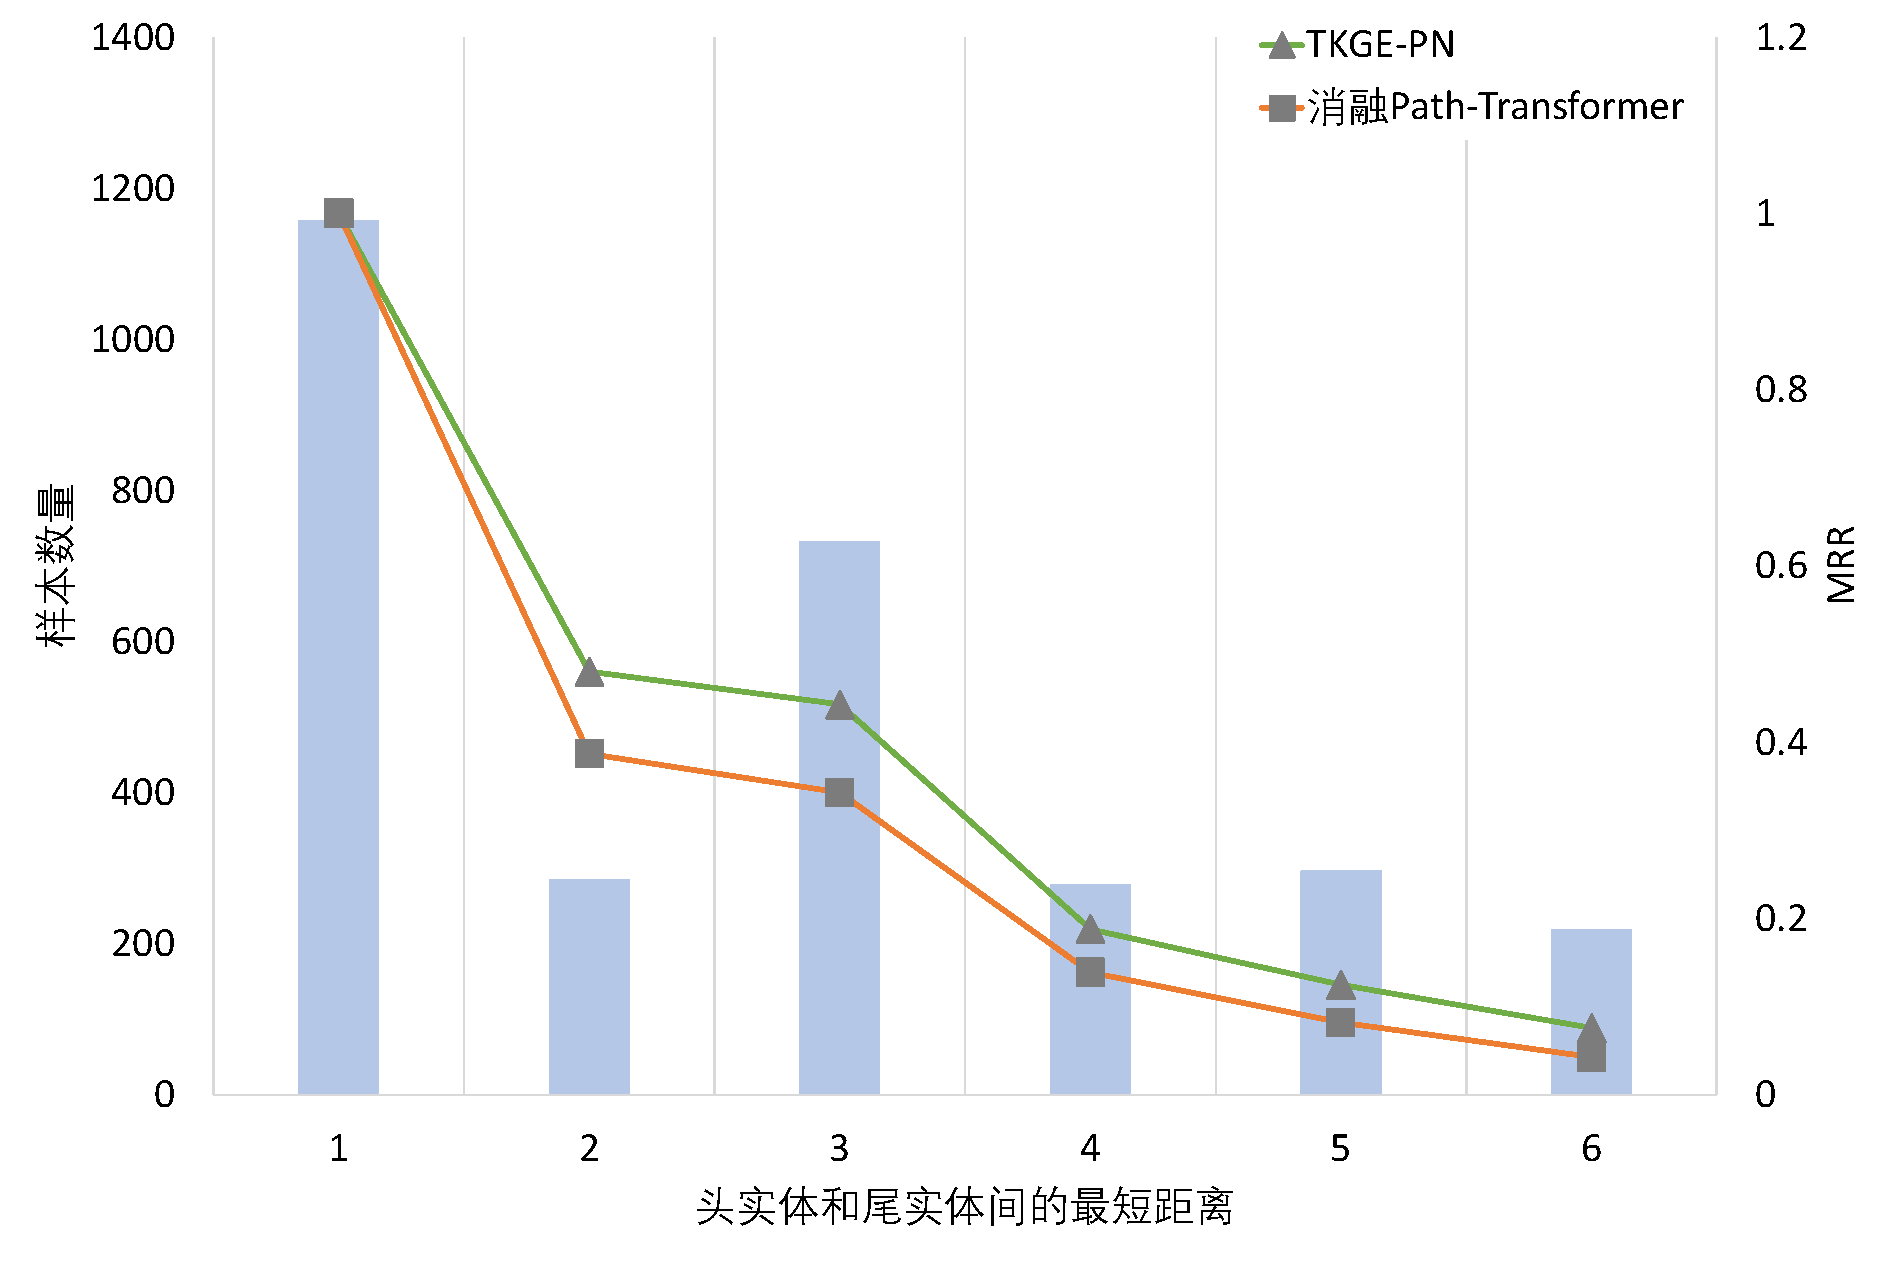
\includegraphics[width=1\textwidth]{pic/TKGE-PN_experiment.pdf}}
    \caption{WN18RR分组实验结果}
    \label{tkge_experiment}
  \end{figure}

从图\ref{tkge_experiment}中实验结果可以发现,随着头实体和尾实体之间最短距离的增加,模型的MRR指标出现了明显的下降,说明推断图谱之间的长距离依赖是非常困难的。 此外,可以注意到的是,相比于消融了图路径编码模块的模型,学习了图路径的TKGE-PN模型在长距离的样本上性能表现更好,特别是在头尾实体间最短距离为2-4的样本上,证明了图路径信息能够有效捕捉实体间的长距离依赖,提高链路预测任务的性能表现。

\section{本章小结}

本章对于结合图路径和局部邻域的Transformer模型TKGE-PN的实验部分进行了介绍,首先介绍了用来对比的基线模型以及模型在两个数据集上的超参数设置。之后论文对TKGE-PN模型的整体实验结果进行了介绍,证明了TKGE-PN模型性能表现优于绝大部分现有的模型。论文随后通过实验进一步探究了路径长度以及路径采样策略对于TKGE-PN性能的影响;最后论文通过实验对TKGE-PN模型中的关键设计进行了具体的探究和分析,包括图路径编码模块、局部邻域编码模块以及掩蔽实体关系预测任务,并设计了实验证明了图路径在长距离依赖信息学习中的重要作用。